\chapter{MEMBUAT DATA SPASIAL (DIGITASI)}

Sebelumnya kita telah belajar bagaimana membuat peta sederhana dengan menampilkan Data Spasial yang telah disediakan. Tetapi, kita juga harus mempelajari bagaimana membuat Data Spasial yang baru, terutama jika kita tidak mempunyai Data Spasial tersebut. Misalkan, kita mempunyai sumber data \textit{raster} seperti citra satelit, foto udara, peta rupa bumi Indonesia, atau peta lainnya yang memiliki informasi koordinat, kita dapat membuat data spasialnya dengan melakukan digitasi terhadap data \textit{raster} tersebut.

\section{Pengertian Digitasi Peta}

Digitasi secara umum dapat didefinisikan sebagai proses konversi data analog ke dalam format digital. Objek-objek tertentu seperti jalan, rumah, sawah, dan lain-lain yang sebelumnya dalam format \textit{raster} maka menjadi objek-objek \textit{vektor}. Pada sebuah citra satelit resolusi tinggi dapat diubah kedalam format digital dengan proses digitasi.

\section{Metode Digitasi}

Proses digitasi secara umum dibagi dalam dua macam :

\begin{enumerate}[1.]

  \item Digitasi menggunakan \textit{digitizer} (zaman dulu, tetapi kini hampir tidak lagi), dalam proses digitasi ini memerlukan sebuah meja digitasi atau \textit{digitizer}.
  
  \item Digitasi \textit{on-screen} di layar monitor.
  
  Digitasi \textit{on-screen} paling sering dilakukan karena lebih mudah dilakukan, tidak memerlukan tambahan peralatan lainnya, dan lebih mudah untuk dikoreksi apabila terjadi kesalahan.
  
  Digitasi \textit{on-screen} biasanya dilakukan pada/dibantu oleh suatu \textit{base-layer} yang memiliki referensi spasial, misalnya citra satelit.

\end{enumerate}

\section{Membuat \textit{Shapefile}}

\begin{enumerate}[1.]

  \item Untuk membuat \textit{shapefile} baru pada QGIS, pilih menu \texttt{Layer > Create Layer > New Shapefile Layer} seperti pada gambar \ref{fig:menunewshape} atau dengan \textit{shortcut} \texttt{Ctrl + Shift + N}.
  
  \begin{figure}[H]
    \centering
    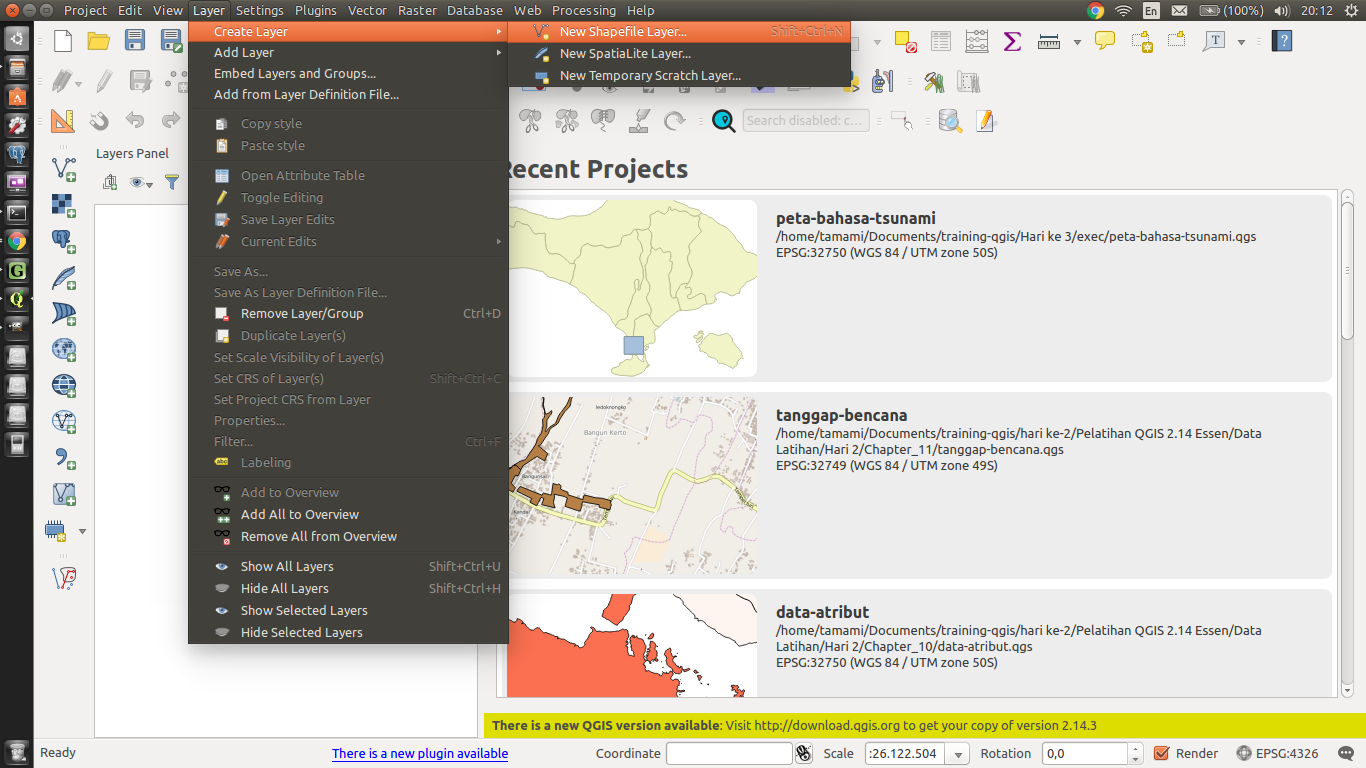
\includegraphics[width=1\textwidth]{./resources/036-menu-new-shape}
    \caption{Menu Menambahkan \textit{Layer Shapefile}}
    \label{fig:menunewshape}
  \end{figure}
  
  \item Kemudian akan muncul kotak dialog pembuatan \textit{layer} baru seperti gambar \ref{fig:newshapedialog}
  
  \begin{figure}[H]
    \centering
    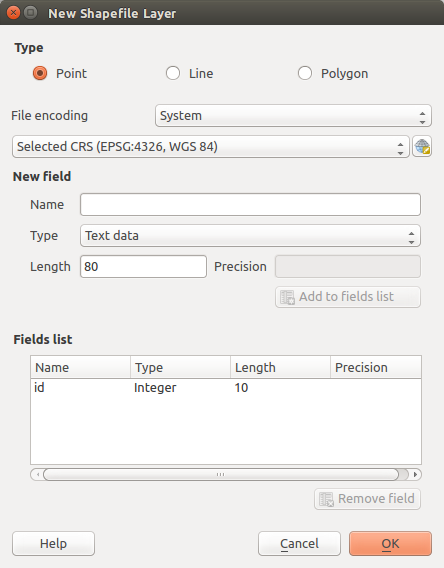
\includegraphics[width=1\textwidth]{./resources/037-new-shape-dialog}
    \caption{Jendela Pembuatan \textit{Layer Shapefile}}
    \label{fig:newshapedialog}
  \end{figure}
  
  Tipe \textbf{Point} adalah jenis \textit{layer} berupa titik yang digunakan untuk membuat \textit{Point of Interest}
  
  Tipe \textbf{Line} adalah jenis \textit{layer} berupa garis digunakan untuk membuat jalan, sungai, dan lainnya.
  
  Tipe \textbf{Polygon} adalah jenis \textit{layer} berupa area/luasan digunakan untuk membuat batas administrasi, \textit{landcover}, bangunan, dan lainnya.
  
  \item Tentukan sistem koordinatnya, di Indonesia sistem koordinat yang dipakai adalah WGS 1984. Apabila ingin menggunakan sistem koordinat UTM dengan zona UTM yang tentunya wilayah Kabupaten Brebes berada pada WGS84 UTM 49S (sebagai referensi tentang sistem koordinat yang digunakan, dapat melihat kembali bab tentang sistem koordinat).
  
  \item Membuat kolom pada data atribut.
  
  \begin{itemize}
  
    \item Buat nama kolom pada bagian \textit{Name}
    
    \item Tentukan tipe data yang ingin digunakan pada bagian \textit{Type}, keterangan untuk tiap tipe data adalah sebagai berikut :
    
    \begin{enumerate}[a.]
    
      \item \textbf{Tipe Data \textit{Text / String}} merupakan jenis data berupa teks, seluruh karakter termasuk \textit{alphanumeric} yang berjumlah maksimal 255 karakter.
      
      \item \textbf{Tipe Data \textit{Whole Number / Integer}} merupakan jenis data untuk bilangan bulat, seluruh angka termasuk positif dan negatif yang biasanya digunakan untuk menunjukkan nilai banyak (kuantitas) dari suatu tema, misalnya populasi penduduk.
      
      \item \textbf{Tipe Data \textit{Decimal Number / Real}} merupakan jenis data untuk bilangan pecahan yang biasa dituliskan dalam bentuk desimal dan memiliki \textit{range} yang spesifik. Dengan menggunakan tipe data ini, kita bisa 'menolak' sebuah nilai jika nilai tersebut diluar dari \textit{precision} dan \textit{scale} yang sudah ditentukan sebelumnya. Contoh : Kita menentukan \textit{precision} 4 (lebar \textit{field} hanya menerima maksimal 4 angka termasuk nilai \textit{decimal} tanpa memperhitungkan pemecahan angka tersebut, yaitu titik sebagai bentuk desimal) dan \textit{scale} 2 (maksimal 2 angka setelah pemecah angka tersebut, yaitu titik sebagai bentuk desimal), maka \textit{field} tersebut bisa menerima nilai 12,35 tetapi tidak dapat menerima nilai-nilai 1,235 dan 123,5. 
    
    \end{enumerate}
    
    \item Atur panjangnya karaketer yang dapat disimpan pada kolom \textit{width}.
    
    \item Khusus untuk tipe data \textit{Decimal Number} kita bisa mengatur panjangnya karakter sesudah koma yang dapat disimpan pada kolom \textit{Precision}
    
    \item Sebagai catatan saja bahwa nama \textit{field} terbatas hanya 10 karaketer saja dan hanya bisa menggunakan huruf, angka, \textit{hypens}, dan \textit{underscore}. Sepasang karakter dibolehkan tetapi tidak disarankan. Tidak bisa memberi nama \textit{field} menggunakan spasi atau spesial karakter lainnya, misalnya tanda tanya (?).
    
    \item Nama \textit{shapefile} boleh maksimal 10 karaketer (huruf, angka, underscore "\_").
  
  \end{itemize}
  
  \item Apabila sudah terisi semua, baik dari nama \textit{field}, tipe data, dan panjangnya data, kemudian klik \texttt{Add to fields list} untuk menambahkan daftar atribut yang akan dipasangkan pada \textit{shapefile} yang dibuat.
  
  \item Jika sudah selesai, tekan tombol \verb|OK| sehingga muncul jendela untuk menyimpan \textit{file} untuk \textit{layer shapefile} ini.

\end{enumerate}

Penentuan nama \textit{file} dan atributnya sudah dijadikan standar dengan penjelasan sebagai berikut :

\begin{itemize}

  \item \textit{Layer} Tanah / Bidang
  
  \textit{Layer} ini berisi tanah / bidang objek pajak dalam satu Desa / Kelurahan, dimana penamaan \textit{file} untuk layer tanah / bidang mengikuti format \texttt{3329KKKLLL}, dimana polanya adalah sebagai berikut :
  
  \begin{itemize}
    \item \texttt{33} adalah 2 (dua) digit kode Propinsi Jawa Tengah, sehingga sifatnya mutlak.
    \item \texttt{29} adalah 2 (dua) digit kode Kabupaten Brebes, sehingga sifatnya mutlak.
    \item \texttt{KKK} adalah 3 (tiga) digit kode Kecamatan di Kabupaten Brebes yang dapat dilihat pada basis data SISMIOP sebagai referensi.
    \item \texttt{LLL} adalah 3 (tiga) digit kode Kelurahan/Desa di Kabupaten Brebes yang dapat dilihat pada basis data SISMIOP sebagai referensi.
  \end{itemize}
  
  \textit{Layer} ini bertipe \textbf{poligon}, dengan \textit{fill patter} \textbf{none}, \textit{border style} \textbf{garis penuh}, \textit{color} \textbf{black} dan \textit{width} \textbf{0,17mm}. 
  
  Struktur data yang ada pada \textit{layer} tanah / bidang ini adalah seperti pada tabel berikut :
  
  \begin{table}[H]
    \centering
    \begin{tabular}{| c | c | c | p{7cm} |}
      \hline
      Field & Tipe & Index & Keterangan \\
      \hline \hline
      \textbf{d\_nop} & character(18) & index1 & NOP setiap bidang tanah \\
      \hline
      \textbf{d\_luas} & decimal(10,2) & & luas bidang tanah dengan menggunakan update kolom terhadap \textit{field} d\_luas dengan \textit{field calculator} \\
      \hline
    \end{tabular}
  \end{table}
  
  \item \textit{Layer} Bangunan
  
  \textit{Layer} ini berisi gambar denah bangunan dalam satu Desa/Kelurahan, dimana penamaan \textit{file} mengikuti aturan \texttt{3329KKKLLLbg}, dimana polanya adalah sebagai berikut :
  
  \begin{itemize}
    \item \texttt{33} adalah 2 (dua) digit kode Propinsi Jawa Tengah, sifatnya mutlak.
    \item \texttt{29} adalah 2 (dua) digit kode Kabupaten Brebes, sifatnya mutlak.
    \item \texttt{KKK} adalah 3 (tiga) digit kode Kecamatan yang dapat dilihat pada basis data SISMIOP sebagai referensi.
    \item \texttt{LLL} adalah 3 (tiga) digit kode Kelurahan yang dapat dilihat pada basis data SISMIOP sebagai referensi.
  \end{itemize}
  
  \textit{Layer} ini memiliki ciri fisik lain yaitu bertipe \textbf{poligon}, dengan \textit{fill pattern} seperti \textbf{MapInfo no. 5}, \textit{foreground} seperti \textbf{MapInfo no. 7}, \textit{background} \textbf{none}, \textit{border style} \textbf{garis putus}, \textit{line style} seperti \textbf{MapInfo no. 5}, \textit{color} \textbf{hijau}, dan \textit{width} \textbf{0,17mm}.
  
  Struktur basis data untuk \textit{layer} bangunan ini adalah sebagai berikut :
  
  \begin{table}[H]
    \centering
    \begin{tabular}{| c | c | c | p{7cm} |}
      \hline
      Field & Tipe & Index & Keterangan \\
      \hline\hline
      \textbf{d\_nop} & character(21) & index1 & NOP ditambah nomor bangunan untuk tiap bangunannya \\
      \hline
    \end{tabular}
  \end{table}
  
  \item \textit{Layer} Jalan
  
  \textit{Layer} jalan ini berisi gambar jalan dalam satu Desa/Kelurahan, dimana penamaan \textit{file} untuk \textit{layer} ini mengikuti aturan \texttt{3329KKKLLLjl}, dengan keterangan sebagai berikut :
  
  \begin{itemize}
    \item \texttt{33} adalah 2 (dua) digit kode Propinsi Jawa Tengah.
    \item \texttt{29} adalah 2 (dua) digit kode Kabupaten Brebes.
    \item \texttt{KKK} adalah 3 (tiga) digit kode Kecamatan yang dapat dilihat pada basis data SISMIOP sebagai referensi.
    \item \texttt{LLL} adalah 3 (tiga) digit kode Kelurahan yang dapat dilihat pada basis data SISMIOP sebagai referensi.
  \end{itemize}
  
  \textit{Layer} ini memiliki ciri fisik yaitu bertipe \textbf{Polyline}, \textit{style} \textbf{garis penuh}, \textit{color} \textbf{red}, \textit{width} \textbf{0,17mm}.
  
  Struktur basis data untuk \textit{layer} jalan ini adalah sebagai berikut :
  
  \begin{table}[H]
    \centering
    \begin{tabular}{| c | c | c | p{7cm} |}
      \hline
      Field & Tipe & Index & Keterangan \\
      \hline\hline
      \textbf{d\_nm\_jln} & character(30) & & Nama Jalan \\
      \hline
      \textbf{d\_lbr\_jln} & Integer & & Lebar jalan (rata-rata lebar pada jalan tersebut) \\
      \hline
    \end{tabular}
  \end{table}
  
  \item \textit{Layer} Sungai
  
  \textit{Layer} ini berisi gambar sungai dalam satu Desa/Kelurahan, dimana penamaan \textit{file} untuk \textit{layer} ini mengikuti aturan \texttt{3329KKKLLLsg}, dengan keterangan berikut :
  
  \begin{itemize}
    \item \texttt{33} adalah 2 (dua) digit kode Propinsi Jawa Tengah.
    \item \texttt{29} adalah 2 (dua) digit kode Kabupaten Brebes
    \item \texttt{KKK} adalah 3 (tiga) digit kode Kecamatan yang dapat dilihat pada basis data SISMIOP sebagai referensi
    \item \texttt{LLL} adalah 3 (tiga) digit kode Kelurahan yang dapat dilihat pada basis data SISMIOP sebagai referensi.
  \end{itemize}
  
  \textit{Layer} ini memiliki ciri fisik bertipe \textbf{polyline}, dengan \textit{style} \textbf{garis penuh}, \textit{color} \textbf{blue}, dan \textit{width} \textbf{0,17mm}.
  
  Struktur basis data untuk \textit{layer} sungai ini adalah sebagai berikut :
  
  \begin{table}[H]
    \centering
    \begin{tabular}{| c | c | c | p{7cm} |}
      \hline
      Field & Tipe & Index & Keterangan \\
      \hline\hline
      \textbf{d\_nm\_sng} & character(30) & & Nama Sungai \\
      \hline
      \textbf{d\_lbr\_sng} & integer & & Lebar sungai (rata-rata lebar pada sungai tersebut) \\
      \hline
    \end{tabular}
  \end{table}
  
  \item \textit{Layer} Teks
  
  \textit{Layer} ini berisi keterangan teks dalam satu Desa/Kelurahan, penamaan \textit{file} untuk \textit{layer} ini mengikuti aturan \texttt{3329KKKLLLtx}, dengan keterangan sebagai berikut :
  
  \begin{itemize}
    \item \texttt{33} adalah 2 (dua) digit kode Propinsi Jawa Tengah
    \item \texttt{29} adalah 2 (dua) digit kode Kabupaten Brebes
    \item \texttt{KKK} adalah 3 (tiga) digit kode Kecamatan yang dapat dilihat pada basis data SISMIOP
    \item \texttt{LLL} adalah 3 (tiga) digit kode Kelurahan yang dapat dilihat pada basis data SISMIOP.
  \end{itemize}
  
  Struktur basis data untuk \textit{layer} teks ini adalah sebagai berikut :
  
  \begin{table}[H]
    \centering
    \begin{tabular}{| c | c | c | p{7cm} |}
      \hline
      Field & Tipe & Index & Keterangan \\
      \hline\hline
      \textbf{d\_text} & character(30) & & Sebagai penjelas / keterangan pada bidang cetak peta. \\
      \hline
    \end{tabular}
  \end{table}
  
  Kolom \texttt{d\_text} dapat berisi :
  
  \begin{itemize}
    \item Teks mengenai keseluruhan nama utilitas jalan, sungai, informasi nama wilayah yang bersebelahan, informasi lokasi penting, dan sebagainya, yang tidak termasuk \textit{layer-layer} lain berwarna hitam dengan tipe huruf \textit{italic} berukuran sesuai dengan gambar.
    \item Batas tepi jalan diperkeras berwarna merah ukuran garis paling tipis
    \item Batas tepi jalan tidak diperkeras berwarna coklat kekuningan berukuran garis paling tipis
    \item Batas tepi jalan TOL berwarna merah berukuran garis tipis nomor 2 (di MapInfo)
    \item Batas tepi sungai berwarna biru berukuran garis tipis nomor 2 (di MapInfo).
    \item Utilitas yang disertai dengan simbolnya.
  \end{itemize}
  
  \item \textit{Layer} Batas Blok
  
  \textit{Layer} ini menggambarkan batas blok dalam suatu Desa/Kelurahan, penamaan \textit{file} mengikuti aturan \texttt{3329KKKLLLbl} dengan keterangan sebagai berikut :
  
  \begin{itemize}
    \item \texttt{33} adalah 2 (dua) digit kode Propinsi Jawa Tengah
    \item \texttt{29} adalah 2 (dua) digit kode Kabupaten Brebes
    \item \texttt{KKK} adalah 3 (tiga) digit kode Kecamatan yang dapat dilihat pada basis data SISMIOP
    \item \texttt{LLL} adalah 3 (tiga) digit kode Kelurahan yang dapat dilihat pada basis data SISMIOP.
  \end{itemize}
  
  Ciri fisik dari \textit{layer} batas blok ini adalah bertipe \textbf{polygon}, \textit{fill pattern} \textbf{none}, \textit{border style} \textbf{garis putus dan titik}, \textit{line style} \textbf{setara MapInfo nomor 13}, \textit{color} \textbf{blue}, \textit{width} \textbf{0,25mm}.
  
  Dengan struktur basis datanya adalah sebagai berikut :
  
  \begin{table}[H]
    \centering
    \begin{tabular}{| c | c | c | p{7cm} |}
      \hline
      Field & Tipe & Index & Keterangan \\
      \hline\hline
      \textbf{d\_blok} & character(13) & index1 & Kode wilayah + Nomor blok \\
      \hline
    \end{tabular}
  \end{table}
  
  \item \textit{Layer} Simbol
  
  \textit{Layer} ini digunakan untuk memberikan simbol simbol umum pada peta dalam satu Desa/Kelurahan. Penamaan \textit{file} untuk \textit{layer} ini mengikuti aturan \texttt{3329KKKLLLsi}, dengan keterangan sebagai berikut :
  
  \begin{itemize}
    \item \texttt{33} adalah 2 (dua) digit kode Propinsi Jawa Tengah
    \item \texttt{29} adalah 2 (dua) digit kode Kabupaten Brebes
    \item \texttt{KKK} adalah 3 (tiga) digit kode Kecamatan yang dapat dilihat pada basis data SISMIOP.
    \item \texttt{LLL} adalah 3 (tiga) digit kode Kelurahan yang dapat dilihat pada basis data SISMIOP.
  \end{itemize}
  
  Struktur basis data dari \textit{layer} simbol ini adalah sebagai berikut :
  
  \begin{table}[H]
    \centering
    \begin{tabular}{| c | c | c | p{7cm} |}
      \hline
      Field & Tipe & Index & Keterangan \\
      \hline\hline
      \textbf{d\_kd\_simbol} & character(4) & & Kode simbol \\
      \hline
    \end{tabular}
  \end{table}
  
  Dimana isi untuk \textit{field} \texttt{d\_kd\_simbol} adalah :
  
  \begin{table}[H]
    \centering
    \begin{tabular}{| c | c |}
      \hline
      Kode Simbol & Uraian Simbol \\
      \hline\hline
      1 & Kuburan Islam \\
      \hline
      2 & Kuburan Kristen \\
      \hline
      3 & Kuburan lainnya \\
      \hline
      4 & Masjid \\
      \hline
      5 & Gereja \\
      \hline
      6 & Candi \\
      \hline
      7 & Pura / Puri \\
      \hline
      8 & Klenteng \\
      \hline
      9 & Kantor \\
      \hline
      10 & Titik triangulasi \\
      \hline
      11 & Tugu / Titik poligon \\
      \hline
    \end{tabular}
  \end{table}
  
  \item \textit{Layer} Batas Kelurahan
  
  \textit{Layer} ini berisi gambar batas wilayah administrasi tiap Desa/Kelurahan dalam satu Kecamatan. Penamaan \textit{file} untuk \textit{layer} ini mengikuti aturan \texttt{3329KKK} dengan keterangan sebagai berikut :
  
  \begin{itemize}
      \item \texttt{33} adalah 2 (dua) digit kode Propinsi Jawa Tengah
      \item \texttt{29} adalah 2 (dua) digit kode Kabupaten Brebes
      \item \texttt{KKK} adalah 3 (tiga) digit kode Kecamatan.
  \end{itemize}
  
  Adapun ciri dari \textit{layer} batas kelurahan ini adalah bertipe \textbf{poligon}, \textit{fill pattern} \textbf{none}, \textit{border style} \textbf{garis putus} dengan \textit{line style} seperti \textbf{MapInfo Nomor 7}, \textit{color} \textbf{black}, dengan \textit{width} \textbf{1 mm}.
  
  Struktur basis data untuk \textit{layer} batas administrasi Kelurahan adalah sebagai berikut :
  
  \begin{table}[H]
    \centering
    \begin{tabular}{| c | c | c | p{7cm} |}
      \hline
      Field & Tipe & Index & Keterangan \\
      \hline\hline
      \textbf{d\_kd\_kel} & character(10) & index1 & Kode wilayah Kelurahan \\
      \hline
      \textbf{d\_nm\_kel} & character(25) & & Nama Kelurahan \\
      \hline
    \end{tabular}
  \end{table}
  
  \item \textit{Layer} Batas Kecamatan
  
  \textit{Layer} ini berisi gambar batas administrasi untuk tiap Kecamatan dalam 1 (satu) Kabupaten/Kota. Penamaan \textit{file} untuk \textit{layer} ini hanya \texttt{3329}, karena gambarnya hanya berisi batas administrasi Kecamatan di Kabupaten Brebes.
  
  \textit{Layer} ini memiliki ciri bertipe \textbf{poligon}, \textit{fill pattern} \textbf{none}, \textit{border style} \textbf{garis putus} dengan \textit{line style} seperti \textbf{MapInfo Nomor 7}, \textit{color} \textbf{black}, dan \textit{width} \textbf{1 mm}.
  
  Struktur basis data untuk \textit{layer} batas administrasi Kecamatan adalah sebagai berikut :
  
  \begin{table}[H]
    \centering
    \begin{tabular}{| c | c | c | p{7cm} |}
      \hline
      Field & Tipe & Index & Keterangan \\
      \hline\hline
      \textbf{d\_kd\_kec} & character(7) & index1 & Kode wilayah Kecamatan \\
      \hline
      \textbf{d\_nm\_kec} & character(25) & & Nama Kecamatan \\
      \hline
    \end{tabular}
  \end{table}
  
  \item \textit{Layer} Batas Kabupaten
  
  \textit{Layer} ini berisi gambar batas administrasi Kabupaten, karena wilayah yang dibutuhkan hanya Kabupaten Brebes, maka hanya ada 1 (satu) \textit{file} untuk \textit{layer} ini dengan nama \textit{file} \texttt{33}.
  
  Ciri dari \textit{layer} batas Kabupaten ini bertipe \textbf{poligon}, \textit{fill pattern} \textbf{none}, \textit{border style} \textbf{garis positif} seperti \textit{line style} \textbf{MapInfo nomor 32}, \textit{color} \textbf{black}, dan \textit{width} \textbf{1 mm}.
  
  Struktur basis datanya adalah seperti berikut ini :
  
  \begin{table}[H]
    \centering
    \begin{tabular}{| c | c | c | p{7cm} |}
      \hline
      Field & Tipe & Index & Keterangan \\
      \hline\hline
      \textbf{d\_kd\_dt2} & character(4) & index1 & Kode Wilayah Daerah Kabupaten \\
      \hline
      \textbf{d\_nm\_dt2} & character(25) & & Nama Daerah Kabupaten \\
      \hline
    \end{tabular}
  \end{table}

\end{itemize}

\section{Penentuan Nilai Atribut dengan \textit{Value Map}}

Dalam banyak kasus sebenarnya tidak diperbolehkan mengisi data atribut secara bebas, tetapi harus memilih salah satu dari beberapa pilihan, misalnya dalam pengisian kelas jalan, pilihannya jalan Primer, jalan Sekunder, jalan Tersier, dan lain-lain, atau pada saat pengisian data pada \textit{layer} simbol, maka perlu dibuatkan pilihannya.

Dengan Quantum GIS, kita dapat memberikan pilihan ketika mengisikan data atribut pada \textit{field} tertentu. Dengan menggunakan layer simbol, pada saat akan mengisikan kode simbol sebagai atribut, akan dimunculkan pilihan-pilihan isian dengan langkah-langkah berikut :

\begin{enumerate}[1.]

  \item Pastikan \textit{layer} yang dipilih aktif dan berada pada kondisi edit dengan menekan tombol \textit{Toggle Editing}, atau memilih menu \texttt{Layer > Toggle Editing}
  
  \item Tampilkan \textit{Layer Properties}, dengan klik kanan pada \textit{layer} \texttt{3329160009si} atau memilih menu \texttt{Layer > Properties} seperti pada gambar \ref{fig:layerproperties}.
  
  \begin{figure}[H]
    \centering
    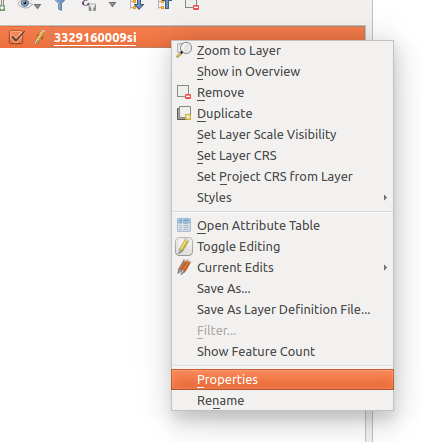
\includegraphics[scale=0.7]{./resources/038-layer-properties}
    \caption{Menu \textit{Layer Properties}}
    \label{fig:layerproperties}
  \end{figure}
  
  \item Pilih bagian \textit{Field}, setelah itu pada kolom \textit{Edit Widget} klik tombol \texttt{Text Edit} untuk kolom \texttt{d\_kd\_simbo} seperti gambar \ref{fig:layerpropertieswin}
  
  \begin{figure}[H]
    \centering
    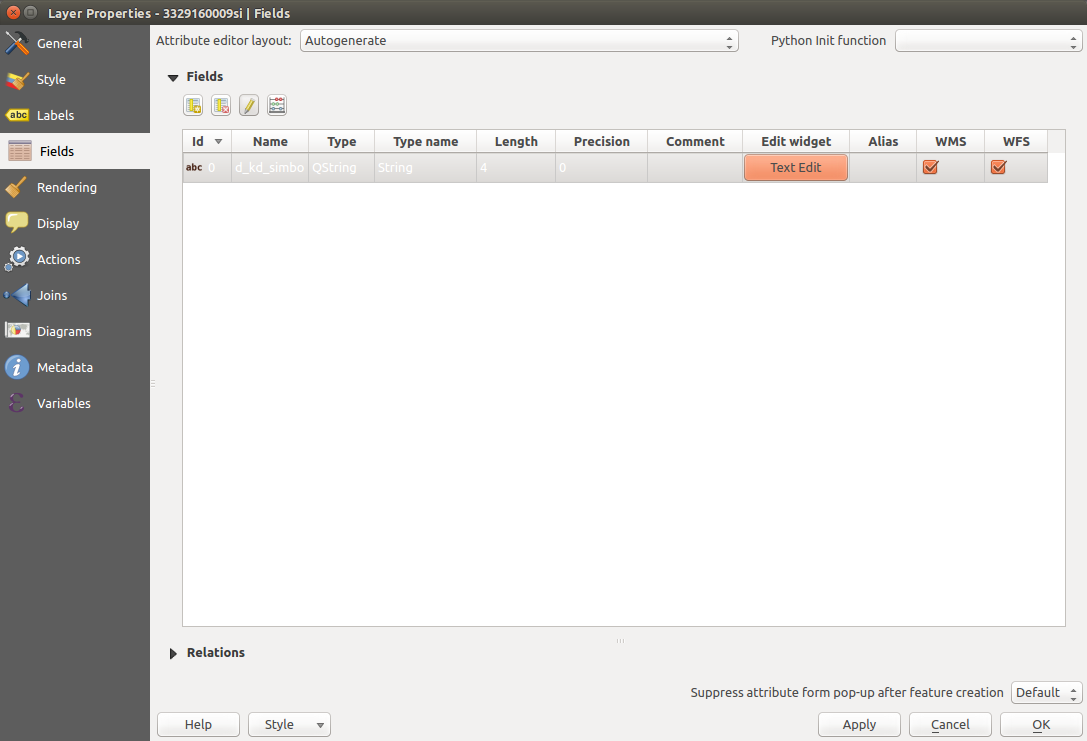
\includegraphics[width=1\textwidth]{./resources/039-jendela-layer-properties}
    \caption{Jendela \textit{Layer Properties}}
    \label{fig:layerpropertieswin}
  \end{figure}
  
  \item Pada menu \textit{Text Edit} pilih \textit{Value Map}, lalu isi nilai sesuai dengan ketentuan pengklasifikasian simbol dihalaman sebelumnya seperti pada gambar \ref{fig:simbolmapping}, klik \texttt{OK} pada kotak dialog \textit{edit attribute} dan klik \texttt{OK} pada menu \textit{field layer properties}.
  
  \begin{figure}[H]
    \centering
    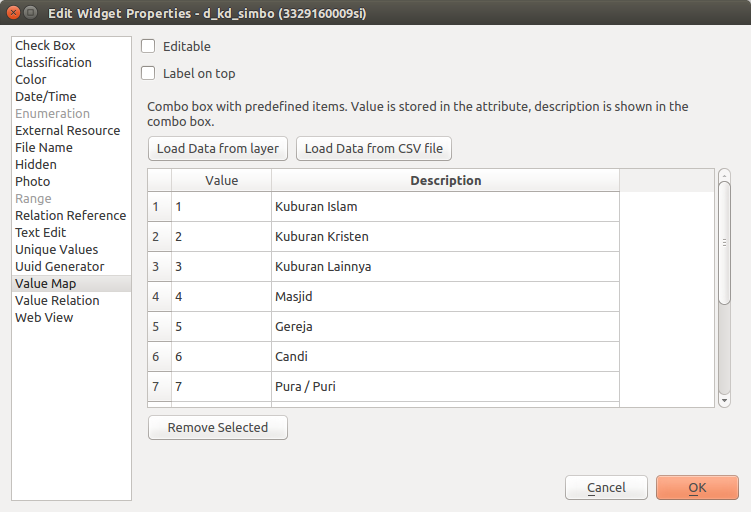
\includegraphics[width=1\textwidth]{./resources/040-mapping-simbol}
    \caption{\textit{Mapping} Simbol Untuk Mempermudah Pengisian}
    \label{fig:simbolmapping}
  \end{figure}
  
  \item Lakukan digitasi sesuai posisi yang diinginkan, dan pada akhir digitasi akan tampil kotak dialog seperti pada gambar \ref{fig:pilihanatribut} yang memungkinkan pengguna memilih isian untuk atribut tertentu.
  
  \begin{figure}[H]
    \centering
    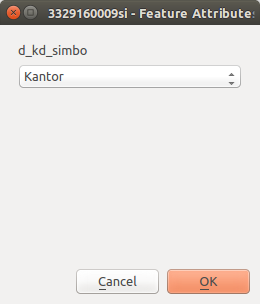
\includegraphics[scale=1]{./resources/041-pilihan-atribut}
    \caption{Pemilihan Isian untuk Atribut}
    \label{fig:pilihanatribut}
  \end{figure}
  
\end{enumerate}

\section{Edit Tabel Atribut}

Kita dapat menambah \textit{field} / kolom pada atribut tabel dengan cara sebagai berikut :

\begin{itemize}

  \item Buka tabel atribut dari \textit{layer} dan mulai mendigitasi dengan klik \textit{toggle editing} seperti pada gambar \ref{fig:iconediting}
  
  \begin{figure}[H]
    \centering
    
\includegraphics[scale=1]{./resources/042-icon-toggle-editing}
    \caption{Ikon \textit{Toggle Editing}}
    \label{fig:iconediting}
  \end{figure}  
  
  \item Kemudian klik \texttt{New Field} seperti pada gambar \ref{fig:iconnewfield}
  
  \begin{figure}[H]
    \centering
    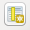
\includegraphics[scale=1]{./resources/043-icon-new-field}
    \caption{Ikon \textit{New Field}}
    \label{fig:iconnewfield}
  \end{figure}
  
  \item Kemudian akan muncul dialog seperti pada gambar \ref{fig:addfielddialog} dan isikan nama \textit{field} / kolom serta tipe data dan keterangan penjelas yang lain.
  
  \begin{figure}[H]
    \centering
    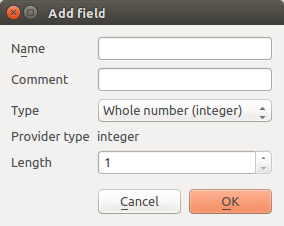
\includegraphics[scale=1]{./resources/044-add-field-dialog}
    \caption{Dialog \textit{Add Field}}
    \label{fig:addfielddialog}
  \end{figure}
  
  \item Setelah semua informasi terisi, klik tombol \texttt{OK}, direkomendasikan untuk klik \textit{toggle editing} dua kali (untuk stop \textit{editing}, kemudian start \textit{editing} lagi) agar kolom langsung disimpan dalam bentuk \textit{shapefile}.

\end{itemize}

Untuk menghapus satu \textit{field} / kolom, klik \textit{delete field} seperti pada gambar \ref{fig:icondeletefield} dan pilih \textit{field} / kolom yang akan dihapus.

\begin{figure}[H]
  \centering
  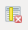
\includegraphics[scale=1]{./resources/045-delete-field-icon}
  \caption{Ikon \textit{Delete Field}}
  \label{fig:icondeletefield}
\end{figure}

Sehingga nantinya akan muncul jendela seperti pada gambar \ref{fig:deletefielddialog}.

\begin{figure}[H]
  \centering
  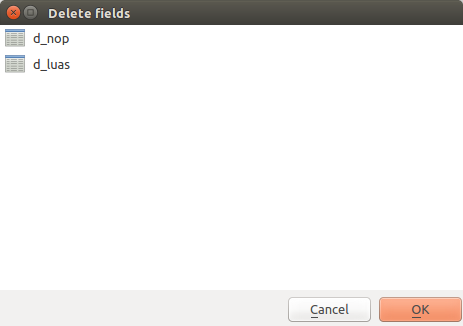
\includegraphics[scale=1]{./resources/046-delete-field-dialog}
  \caption{Dialog \textit{Delete Field}}
  \label{fig:deletefielddialog}
\end{figure}

Setelah itu, apabila kita memilih \textit{toggle editing} atau klik \textit{save edits}, \textit{field} / kolom langsung terhapus dari \textit{shapefile} dan tidak dapat dikembalikan lagi.

Di QGIS belum ada cara untuk bisa mengganti nama \textit{field} / kolom secara langsung.

\section{Memastikan CRS (\textit{Coordinate Reference System}) \textit{Settings}}

Seharusnya CRS (\textit{Coordinate Reference System}) dari \textit{shapefile} dan CRS yang dipilih untuk \textit{Map Project} sama.

\begin{enumerate}[a.]
  \item Lihat CRS pada \textit{shapefile}
  
  Menu: \texttt{layer -> properties... -> tab metadata}
  
  Detailnya akan terlihat seperti pada gambar \ref{fig:crsshapefile}
  
  \begin{figure}[H]
    \centering
    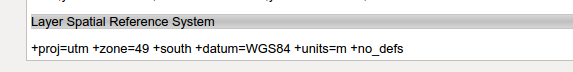
\includegraphics[width=1\textwidth]{./resources/047-crs-shapefile}
    \caption{Informasi CRS \textit{Shapefile} pada \textit{tab Metadata}}
    \label{fig:crsshapefile}
  \end{figure}
  
  \item Melihat CRS untuk \textit{Map Project}
  
  Menu : \texttt{Settings -> Project Properties -> Tab Coordinate Reference System}
\end{enumerate}

  Dipastikan memilih CRS yang sama dengan \textit{layer} yang sedang diedit. Sebagai contoh tampilan CRS \textit{Project} seperti pada gambar \ref{fig:crsproject}.
  
  \begin{figure}[H]
    \centering
    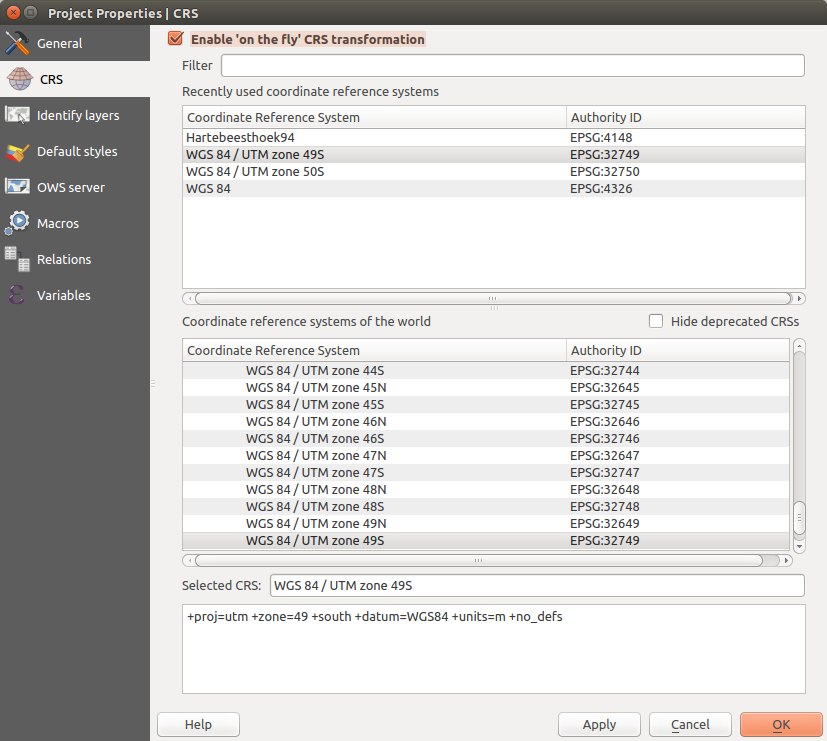
\includegraphics[width=1\textwidth]{./resources/048-crs-project}
    \caption{CRS \textit{Project}}
    \label{fig:crsproject}
  \end{figure}

\section{Memulai Digitasi}

\begin{enumerate}[1.]

  \item Setelah membuat \textit{shapefile} baru, selanjutnya siap untuk dilakukan proses digitasi. Apabila \textit{toolbar digitizing} belum ada, klik \texttt{views > toolbar > digitizing} seperti pada gambar \ref{fig:showdigitizingtoolbar}.
  
  \begin{figure}[H]
    \centering
    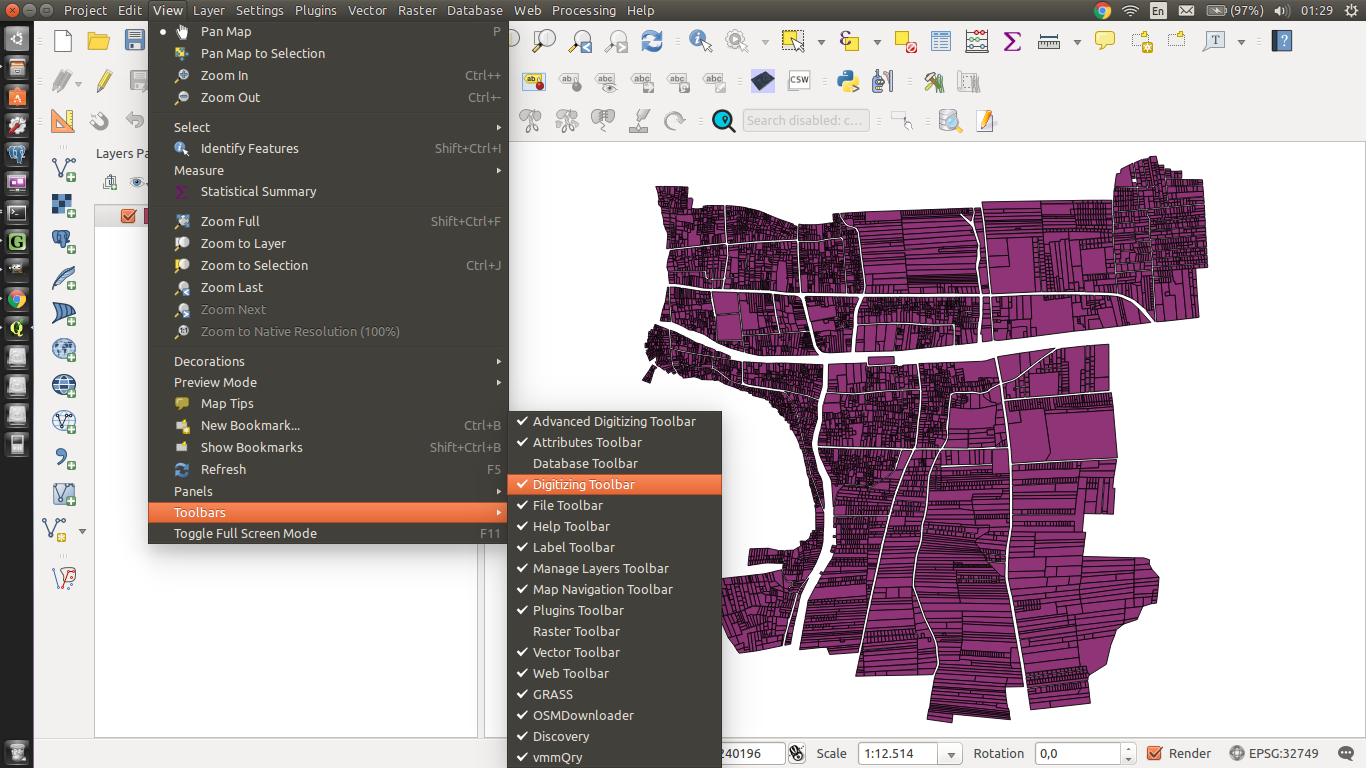
\includegraphics[width=1\textwidth]{./resources/049-show-digitizing-toolbar}
    \caption{Menampilkan \textit{Toolbar Digitizing}}
    \label{fig:showdigitizingtoolbar}
  \end{figure}
  
  \item Untuk mulai mendigitasi, klik \textit{toggle editing}, lalu klik \textit{Add Feature} dengan memilih menu \texttt{Edit > Add Feature}.
  
  \begin{itemize}
    \item Untuk mendigit titik, dapat langsung klik di lokasi yang diinginkan.
    \item Untuk mendigit garis, klik \textit{node-node} garis dengan tombol kiri \textit{mouse} dan klik tombol kanan \textit{mouse} untuk mengakhiri garis.
    \item Untuk mendigit poligon, klik \textit{node-node} poligon dengan tombol kiri \textit{mouse} dan klik tombol kanan \textit{mouse} untuk mengakhiri.
  \end{itemize}
  
  \item Selanjutnya akan muncul kotak dialog pengisian atribut, dapat diisi langsung sesuai data yang ada, atau dapat dikosongkan terlebih dahulu dengan menekan tombol \texttt{OK}
  
  \item Untuk memindahkan fitur yang telah dibuat, dapat menggunakan tombol \textit{Move Feature(s)}, seperti pada gambar \ref{fig:movefeatureicon}.
  
  \begin{figure}[H]
    \centering
    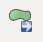
\includegraphics[scale=1]{./resources/050-move-feature-icon}
    \caption{Ikon \textit{Move Feature}}
    \label{fig:movefeatureicon}
  \end{figure}
  
  \item Bila ingin merubah bentuk poligon / garis, dapat menggunakan \textit{Node Tool} seperti pada gambar \ref{fig:nodetoolicon}, kemudian klik di garis poligon sehingga tampak \textit{node} penyusun poligon yang dapat dipindahkan dengan cara tahan klik dan tarik \textit{node} sehingga poligon / garis berubah bentuk.
  
  \begin{figure}[H]
    \centering
    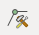
\includegraphics[scale=1]{./resources/051-node-tool-icon}
    \caption{Ikon \textit{Node Tool}}
    \label{fig:nodetoolicon}
  \end{figure}
  
  \item Bila ingin menambahkan \textit{node}, maka cukup klik dua kali pada garis poligon.
  
  \item Untuk menghapus \textit{node} cukup mudah, hanya dengan klik \textit{node} yang akan dihapus, kemudian tekan tombol \texttt{delete} pada \textit{keyboard}.

\end{enumerate}

\section{\textit{Snapping Option}}

Dengan menggunakan fungsi \textit{snap}, kita dapat dengan mudah melakukan digitasi karena dengan fungsi ini dapat melekatkan objek yang dibuat dengan objek lainnya secara otomatis. Untuk pengaturan fungsi \textit{snap} yang akan digunakan pada proses digitasi, dapat diaktifkan pada menu \textit{snapping option} dengan melakukan langkah-langkah berikut :

\begin{enumerate}[1.]
  \item Klik \texttt{setting > snapping option} seperti pada gambar \ref{fig:snappingoptionmenu}.
  
  \begin{figure}[H]
    \centering
    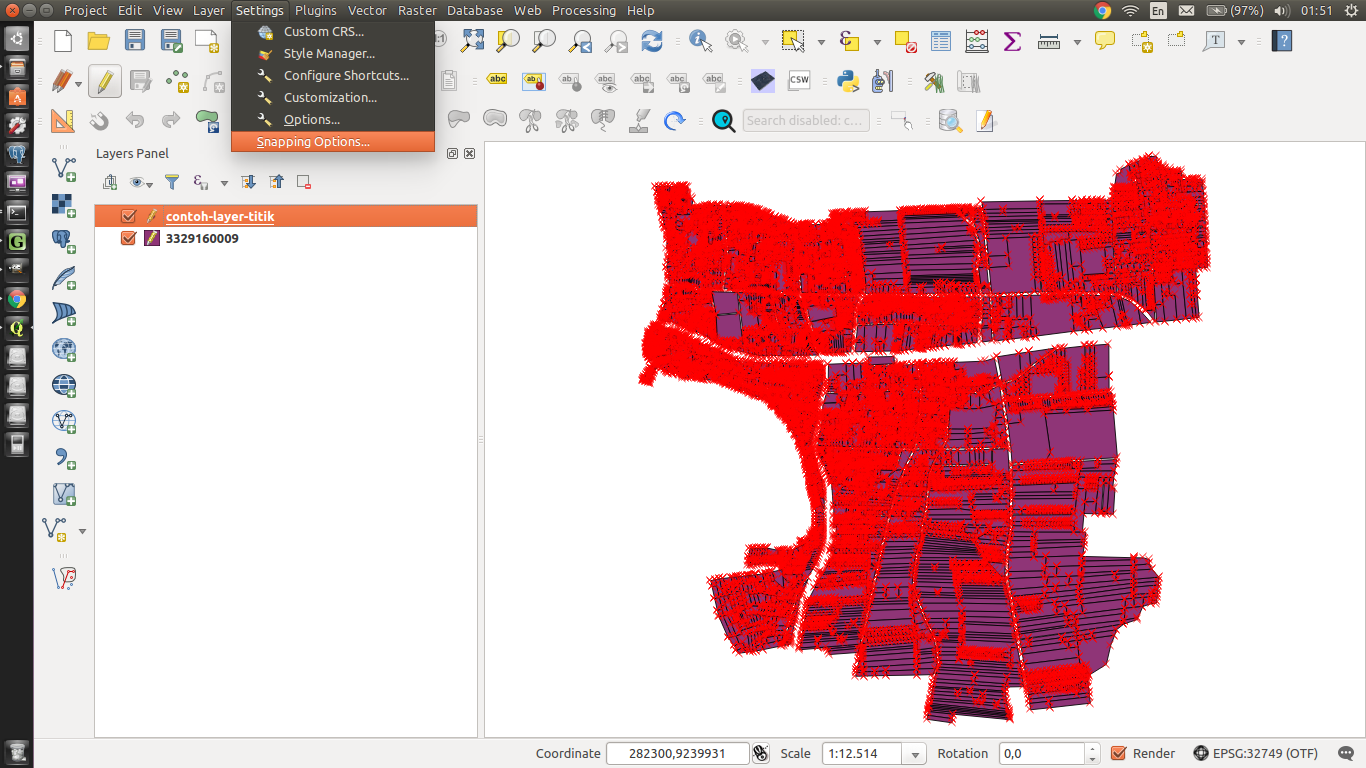
\includegraphics[width=1\textwidth]{./resources/052-snapping-option-menu}
    \caption{Menu \textit{Snapping Option}}
    \label{fig:snappingoptionmenu}
  \end{figure}
  
  \item Kemudian akan muncul kotak dialog seperti pada gambar \ref{fig:snappingdialog}.
  
  \begin{figure}[H]
    \centering
    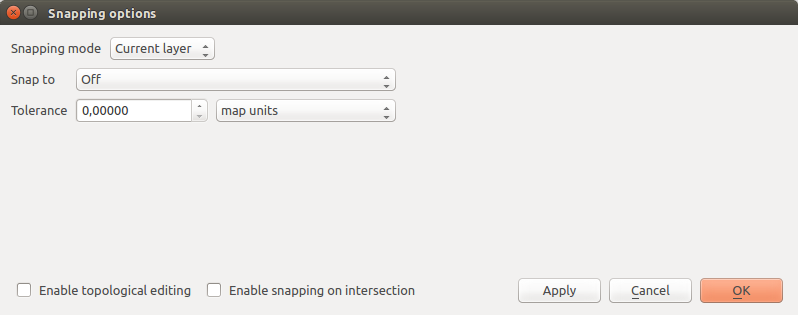
\includegraphics[width=1\textwidth]{./resources/053-snapping-dialog}
    \caption{Dialog \textit{Snapping Option}}
    \label{fig:snappingdialog}
  \end{figure}
  
  \item Untuk mengaktifkan fungsi \textit{snap} baik \textit{snap} ke \textit{vertex}, \textit{snap} ke \textit{segment}, atau \textit{snap} ke keduanya, pilih pada bagian \texttt{snap to}.
  
  \item Untuk memilih jenis \textit{snap} yang ingin digunakan terdapat pada kolom \texttt{mode}.
  
  \begin{itemize}
    \item \texttt{To Vertex} artinya kita akan memilih fungsi \textit{snap} pada titik-titik penyusuan suatu garis.
    \item \texttt{To Segment} artinya akan memilih fungsi \textit{snap} pada garis.
    \item \texttt{To Vertex and Segment} artinya memilih fungsi \textit{snap} pada titik dan garis.
  \end{itemize}
  
  \item \textit{Snap tolerance} digunakan sebagai acuan jarak toleransi antar titik untuk melekatkan pada objek \textit{snap} lainnya yang sudah ada sebelumnya. Nilai \textit{default} yang diberikan QGIS adalah 10 \textit{pixel}. Namun dapat dirubah sesuai kebutuhan.
  
  \item Apabila ingin menambahkan suatu poligon pada poligon lain, dan ingin menempel sesuai bentuk poligon sebelumnya dapat dilakukan dengan mengaktifkan fungsi \textit{topological} (\textit{Enable topological editing})
  
\end{enumerate}

Demikianlah petunjuk teknis dasar penggunaan Quantum GIS sebagai sebuah alat untuk melakukan digitasi dasar peta Pajak Bumi dan Bangunan Perdesaan dan Perkotaan. Untuk melakukan analisa data spasial, akan dibuatkan pada buku petunjuk teknis yang terpisah.